\documentclass[10pt, a5paper]{article}
\usepackage{pdfpages}
\usepackage{parallel}
\usepackage[T2A]{fontenc}
\usepackage{ucs}
\usepackage[utf8x]{inputenc}
\usepackage[polish,english,russian]{babel}
\usepackage{hyperref}
\usepackage{rotating}
\usepackage[inner=2cm,top=1.8cm,outer=2cm,bottom=2.3cm,nohead]{geometry}
\usepackage{listings}
\usepackage{graphicx}
\usepackage{wrapfig}
\usepackage{longtable}
\usepackage{indentfirst}
\usepackage{array}
\newcolumntype{P}[1]{>{\raggedright\arraybackslash}p{#1}}
\frenchspacing
\usepackage{fixltx2e} %text sub- and superscripts
\usepackage{icomma} % коскі ў матэматычным рэжыме
\PreloadUnicodePage{4}

\newcommand{\longpage}{\enlargethispage{\baselineskip}}
\newcommand{\shortpage}{\enlargethispage{-\baselineskip}}

\def\switchlang#1{\expandafter\csname switchlang#1\endcsname}
\def\switchlangbe{
\let\saverefname=\refname%
\def\refname{Літаратура}%
\def\figurename{Іл.}%
}
\def\switchlangen{
\let\saverefname=\refname%
\def\refname{References}%
\def\figurename{Fig.}%
}
\def\switchlangru{
\let\saverefname=\refname%
\let\savefigurename=\figurename%
\def\refname{Литература}%
\def\figurename{Рис.}%
}

\hyphenation{admi-ni-stra-tive}
\hyphenation{ex-pe-ri-ence}
\hyphenation{fle-xi-bi-li-ty}
\hyphenation{Py-thon}
\hyphenation{ma-the-ma-ti-cal}
\hyphenation{re-ported}
\hyphenation{imp-le-menta-tions}
\hyphenation{pro-vides}
\hyphenation{en-gi-neering}
\hyphenation{com-pa-ti-bi-li-ty}
\hyphenation{im-pos-sible}
\hyphenation{desk-top}
\hyphenation{elec-tro-nic}
\hyphenation{com-pa-ny}
\hyphenation{de-ve-lop-ment}
\hyphenation{de-ve-loping}
\hyphenation{de-ve-lop}
\hyphenation{da-ta-ba-se}
\hyphenation{plat-forms}
\hyphenation{or-ga-ni-za-tion}
\hyphenation{pro-gramming}
\hyphenation{in-stru-ments}
\hyphenation{Li-nux}
\hyphenation{sour-ce}
\hyphenation{en-vi-ron-ment}
\hyphenation{Te-le-pathy}
\hyphenation{Li-nux-ov-ka}
\hyphenation{Open-BSD}
\hyphenation{Free-BSD}
\hyphenation{men-ti-on-ed}
\hyphenation{app-li-ca-tion}

\def\progref!#1!{\texttt{#1}}
\renewcommand{\arraystretch}{2} %Іначай формулы ў матрыцы зліпаюцца з лініямі
\usepackage{array}

\def\interview #1 (#2), #3, #4, #5\par{

\section[#1, #3, #4]{#1 -- #3, #4}
\def\qname{LVEE}
\def\aname{#1}
\def\q ##1\par{{\noindent \bf \qname: ##1 }\par}
\def\a{{\noindent \bf \aname: } \def\qname{L}\def\aname{#2}}
}

\def\interview* #1 (#2), #3, #4, #5\par{

\section*{#1\\{\small\rm #3, #4. #5}}

\def\qname{LVEE}
\def\aname{#1}
\def\q ##1\par{{\noindent \bf \qname: ##1 }\par}
\def\a{{\noindent \bf \aname: } \def\qname{L}\def\aname{#2}}
}

\switchlang{en}
\begin{document}
\title{Speed-up Solving Linear Systems on Parallel Architectures via Aggregation of Clans}
\author{Dmitry Zaitsev, Odessa, Ukraine\footnote{\url{daze@acm.org}, \url {https://lvee.org/ru/abstracts/298}}}
\maketitle
\begin{abstract}
Varying minimal clan size brings in certain imbalance when solving a linear (Diophantine) system on parallel architectures via composition of its clans using open source software PaAd. The problem is partially mended by dynamic scheduling of jobs. The present paper studies a task of preliminary balancing the clan size via their aggregation represented as a special case of graph partitioning. Due to complexity of the optimization criteria, taking into consideration both the number of equations and the number of variables on two stages of solution -- solving a system for each clan and solving a composition system -- simplified variants of the task are considered and solved using heuristic techniques: a fast bin packing with the first fit on a sorted array algorithm and a multi-objective graph partitioning with software package METIS. Obtained benchmarks show that aggregation of clans brings in an additional 3 times speed-up.
\end{abstract}
\subsection*{Introduction}

The technique for the composition of linear system clans \cite{bib1} has been further developed with regard to modern parallel architectures and applied to speed-up solving systems of linear Diophantine equations \cite{bib2}, open source software package ParAd released \cite{bib3}.

Solving linear systems is a central task of numerical methods. That is why LAPACK \cite{bib4} is one of the most widespread packets in the world which is applied for benchmarks, including modern supercomputers domain.

Diophantine systems are defined over integer numbers and they appear in manifold application areas, for instance in model-checking with Petri nets for verification of networking protocols \cite{bib5}, manufacture control, data encryption, and artificial intelligence \cite{bib6}. Since the \linebreak computational complexity of solving Diophantine systems is higher than for systems over real numbers, methods to speed-up the process are in demand.

It is convenient to represent (sparse) linear systems as Petri net graphs, equations correspond to transitions (rectangles), variables \linebreak correspond to places (circles). A clan is a subset of the system equations \cite{bib1}. In the decomposition graph \cite{bib1}, each vertex corresponds to a clan; vertices are connected in case the corresponding equations contain common variables.

In the present paper, we specify the clan aggregation task as a special case of graph partitioning \cite{bib7} for a weighted graph having two weights of a node and one weight of an edge. The node weights \linebreak correspond to the number of equations and the number of internal variables of a clan while the edge weight corresponds to the number of contact variables connecting a pair of clans. The optimization criterion should take into consideration the complexity of solving systems for clans and solving the composition system.

Here, for hypertorus 4D of size 3 communication structure, 2D example of size 2 follows

\begin{center}
\begin{figure}[h!]
  \centering
  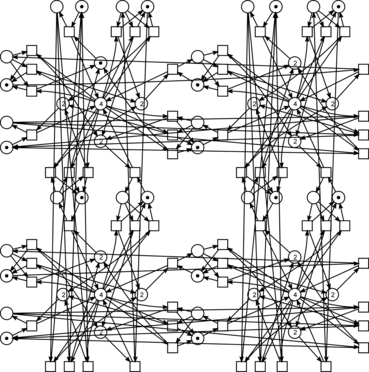
\includegraphics[width=8cm]{Zaitsev1.png}

  \label{fig1}
\end{figure}
\end{center}

\noindent we compare the decomposition graph

\begin{center}
\begin{figure}[h!]
  \centering
  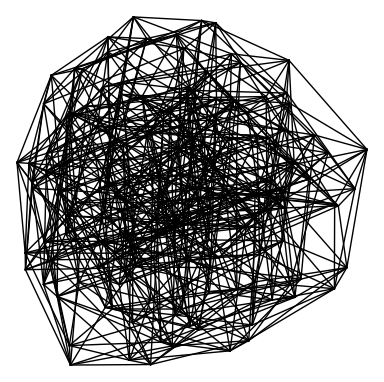
\includegraphics[width=8cm]{Zaitsev2.png}

  \label{fig1}
\end{figure}
\end{center}

\noindent and its aggregation into 7 clans (on the number of available processors minus one)

\begin{center}
\begin{figure}[h!]
  \centering
  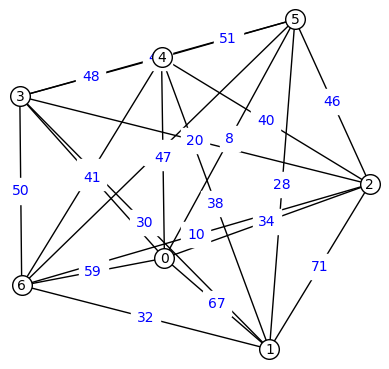
\includegraphics[width=8cm]{Zaitsev3.png}

  \label{fig1}
\end{figure}
\end{center}

A new version of ParAd is released \cite{bib3}, benchmarks for clans \linebreak aggregation are obtained on series of sparse integer matrices which represent Petri net models from Model Checking Contest and \linebreak acknowledged by some tests for real matrices from MatrixMarket and SuiteSparse collections. Aggregation brings-in an additional 3 times speed-up. The speed-up is obtained due to the static load balancing for distributed computing nodes.

\subsection*{Aggregation vs Composition}

We represent the source decomposition of a given system (matrix) into its minimal clans by a weighted graph of the first kind. We use the first kind decomposition graph to aggregate clans for the load balancing. Since at the first stage, a system is solved for each clan, our local goal is to have all the clans merely of the same size. In an ideal case, we need to minimize the number of basis solution as well and this goal is achieved when having merely the same number of equations and variables.

Granulation of the clan technique is limited by the maximal clan size. Thus this value restricts other parameters of the clan aggregation. In other words, when aggregating a subset of clans, the number of equations is summed up while contact variables within sub-graph become internal variables of the aggregated clan, internal variables are summed up as well.

Suppose an aggregated decomposition graph of the first kind is obtained. The first stage of the composition solution of a system is solving a system of equations for each clan. After solving these systems, a decomposition graph of the second kind is obtained. It coincides with the decomposition graph of the first kind with except weights of vertices.

The second kind decomposition graph is employed for either \linebreak simultaneous or sequential or parallel-sequential composition of clans. When a composition system is created, the number of basis solutions (the vertex weights) corresponds to the number of variables while the number of contact variables (the edge weights) corresponds to the number of equations.

The same as for aggregation, the composition operation is \linebreak represented by the sub-graph contraction. Though our goal is to contract a graph into a single vertex finally while for aggregation our goal is to achieve the best edge-cut and the vertex weight balance. That is why the process of composition is called a graph collapse. Recalculation of the vertex weights is reasonable for (parallel-) sequential composition only; for simultaneous composition, it only indicates the number of finally obtained basis solutions.

Thus, after aggregation of clans, the composition process looks the same as described in early works with the only difference we started taking into consideration the vertex weight. In the present paper, we consider global criteria of optimization with regard to the simultaneous composition of clans only. Sequential and parallel-sequential \linebreak composition of clans produce a rather sophisticated sequence of changes for vertex weights and here we do not develop further results on the quasi-optimal collapse of the weighted graph obtained in (for graphs with the edge weights only).

We study the task of clans aggregations separately through global optimization criteria should be considered to choose the proper criterion for aggregation. The global goal consists in minimization of the total time of solving a given system which includes the following stages: decomposition, aggregation, solving systems for clans, composition, \linebreak basis matrix multiplication. In this consideration, we suppose the \linebreak simultaneous composition of clans and the main criterion of \linebreak minimization is the composition system size. For a series of studied systems, exactly a comparably big composition system constituted a bottleneck for the entire process.

\subsection*{Aggregation of Clans via Graph Partitioning using METIS}

A well-known task of k-way graph partitioning is very close to the clan aggregation objectives and METIS \cite{bib7} is one of the best software packages for graph partitioning and it is open source software under Apache 2.0 license. METIS partitions a graph into k parts using either the multilevel recursive bisection or the multilevel k-way partitioning paradigms and achieves rather good performance. It accepts a scalar weight of an edge and a vector of weights for a vertex. The primary METIS objective is the minimization of the edge-cut --- the sum of edge weights of the obtained graph. Besides, it takes into consideration multiple balancing constraints, for instance, the vertex weights equally distributed among the obtained parts.

Thus the primary objective --- the minimal size of composition system --- is completely achieved by METIS while the secondary \linebreak objective of having merely the same size of the clans' systems is achieved partially. Since we can not express transformations of the second vertex weight, we omit it in the decomposition graph specification.

After the decomposition into minimal clans, we compute the number of parts the decomposition graph is partitioned into, and transform the ParAd data structures into METIS API form which is based on the row-compressed representation of a sparse matrix to define the graph adjacency relation and vectors of weights. As a result, METIS produces a vector assigning the partition number to each vertex. According to this vector, the clan decomposition data --- decomposition graph, clans and contact variables specifications --- are reorganized. The rest of ParAd code \cite{bib3} is unchanged: it goes on aggregated clans in the same way as on minimal clans.

\subsection*{Benchmarks for Clans Aggregation}

The following benchmarks have been obtained on cluster Saturn and computer Hare \cite{bib2}. We obtain basic benchmarks solving homogeneous Diophantine systems for Petri net models collection. The following models are considered:

\begin{itemize}
  \item al --- a simplified version of a landing detector for an airplane;
  \item af --- an automatic flight control system;
  \item cd --- a cloud application deployment;
  \item dc --- a distributed language compiler;
  \item ht --- hypertorus communication grid;
  \item sm --- processes sharing memory.
\end{itemize}

The optimum is achieved somewhere in the middle with the number of aggregated clans that provides the merely equal size of the system on two stages of the compositional solution. The two-letter names are used as prefixes in the names of ParAd tests \cite{bib3} and in the following graph where data is measured in the times of speed-ups comparing the ParAd version without aggregation:

\begin{center}
\begin{figure}[h!]
  \centering
  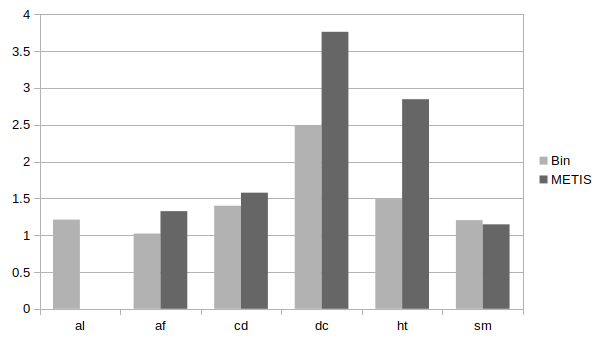
\includegraphics[width=8cm]{Zaitsev4.png}

  \label{fig1}
\end{figure}
\end{center}

METIS \cite{bib7} gives rather good results allowing us to speed-up \linebreak computations a few times, the maximal speed-up of 4 times has been obtained for hypertorus with the higher number of dimensions.

\subsection*{Conclusions}

A series of benchmarks has been obtained for Petri net models and collections of sparse matrices which acknowledge benefits of the developed clan aggregation modules included into a new release of ParAd package \cite{bib3}. Considerable speed-up of 3 times has been obtained solving both Diophantine systems and systems over real numbers.

\subsection*{References}

\begin{thebibliography}{9}
\bibitem{bib1} {Zaitsev D.A. Sequential composition of linear systems’ clans, Information Sciences, Vol. 363, 292–307. http://dx.doi.org/10.1016/j.ins.2016.02.016}
\bibitem{bib2} {Dmitry Zaitsev, Stanimire Tomov, Jack Dongarra. Solving Linear Diophantine Systems on Parallel Architectures, IEEE Transactions on Parallel and Distributed Systems, 30(5), 2019, 1158–1169. http://dx.doi.org/10.1109/TPDS.2018.2873354}
\bibitem{bib3} {ParAd: Solve a linear Diophantine homogeneous (sparse) system via composition of its clans on parallel architectures, https://github.com/dazeorgacm/ParAd}
\bibitem{bib4} {LAPACK — Linear Algebra PACKage, http://www.netlib.org/lapack}
\bibitem{bib5} {Zaitsev D.A. Clans of Petri Nets: Verification of protocols and performance evaluation of networks, LAP LAMBERT Academic Publishing, 2013, 292 p. http://daze.ho.ua/daze-clans-covered-draft.djvu}
\bibitem{bib6} {Zaitsev D.A. Sleptsov Nets Run Fast, IEEE Transactions on Systems, Man, and Cybernetics: Systems, 2016, Vol. 46, No. 5, 682 -- 693. http://dx.doi.org/10.1109/TSMC.2015.2444414}
\bibitem{bib7} {George Karypis. 2019. METIS -- Serial Graph Partitioning and Fill-reducing Matrix Ordering. http://glaros.dtc.umn.edu/gkhome/metis/metis/overview}\end{thebibliography}
\end{document}
